
\documentclass[runningheads,a4paper]{llncs}

\usepackage{graphicx}
\usepackage[space]{grffile}
\usepackage{latexsym}
\usepackage{amsfonts,amsmath,amssymb}
\usepackage{url}
\usepackage[utf8]{inputenc}
\usepackage{hyperref}
\hypersetup{colorlinks=false,pdfborder={0 0 0}}
\usepackage{textcomp}
\usepackage{longtable}
\usepackage{multirow,booktabs}

\usepackage{amssymb}
\setcounter{tocdepth}{3}
%\usepackage{graphicx}

\urldef{\mailsa}\path|{celeste.chudyk, boochs}@hs-mainz.de|
\urldef{\mailsb}\path|{hugo.castaneda, romain.leger, islem.yahiaoui}@iut-dijon.u-bourgogne.fr|
\newcommand{\keywords}[1]{\par\addvspace\baselineskip
\noindent\keywordname\enspace\ignorespaces#1}

\bibliographystyle{splncs03} 




\begin{document}

\mainmatter  % start of an individual contribution

% first the title is needed
\title{Development of an Automatic Pollen Classification System Using Shape,
Texture and Aperture Features}

\titlerunning{Automatic Pollen Classification System}

\authorrunning{Chudyk, Castaneda, Leger, Yahiaoui, Boochs}

\author{Celeste Chudyk\inst{1}, Hugo Castaneda\inst{2}, Romain Leger\inst{2}, Islem Yahiaoui\inst{2}, Frank Boochs\inst{1}%
}

\institute{i3mainz, University of Applied Sciences Mainz, Germany \\
\mailsa\\
\and Dijon Institute of Technology, Burgundy University, France \\
\mailsb
}

\tocauthor{Celeste Chudyk, Hugo Castaneda, Romain Leger, Islem Yahiaoui, Frank Boochs}
\toctitle{Development of an Automatic Pollen Classification System Using Shape, Texture and Aperture Features}
\maketitle



\begin{abstract}
Automatic detection and classification of pollen species has value for use inside of palynologic allergen studies. Traditional labeling of different pollen species requires an expert biologist to classify particles by sight, and is therefore time-consuming and expensive. Here, an automatic process is developed which segments the particle contour and uses the extracted features for the classification process. We consider shape features, texture features and aperture features and analyze which are useful. The texture features analyzed include: Gabor Filters, Fast Fourier Transform, Local Binary Patterns, Histogram of Oriented Gradients, and Haralick features. We have streamlined the process into one code base, and developed multithreading functionality to decrease the processing time for large datasets.
\keywords{Image processing, Machine learning, Pollen, Texture classification}
\end{abstract}

  
  
  
  

\section{Introduction}

Currently, pollen count information is usually limited to generalizing all pollen types with no access to information regarding particular species. In order to differentiate species, typically a trained palynologist would have to manually count samples using a microscope. Advances in image processing and machine learning enable the development of an automatic system that, given a digital image from a bright-field microscope, can automatically detect and describe the species of pollen particles present.

We build upon previous work from within our lab which has planned the structure for a complete personal pollen tracker \cite{Lozano_2012}. For image classification, preliminary results have shown that extraction of both shape features and aperture features lead to useful results \cite{Lozano_2014}. To expand on this research, we have built a software process that not only considers shape and aperture features, but also adds multiple texture features. The range of tested image types has also been greatly expanded in order to build a robust model capable of classifying a highly variable dataset. 

  
  
  
  

\section{Overview} 

The steps for our process are as follows: 1. Image acquisition and particle segmentation, 2. Feature extraction, and 3. Classification.

Our process begins with scanning glass slides of the various pollen species with a digital microscope, then segmenting these images to gather samples of individual pollen particles. These images are then further segmented to identify the pollen boundary, and the area within this boundary is used for feature extraction. 18 shape features, texture features including the Fast Fourier Transform, Local Binary Patterns, Histogram of Oriented Gradients, and Haralick features, as well as aperture features are used. These features are then trained using supervised learning to build a model for the 5 pollen species sampled. The model is then tested with ten-fold cross validation. The process is illustrated in figure \ref{fig:process}. 
    
    
    
    
    
    
    
    
    
    
    
    
  
  
  
  
  
  
  
  
  
  
  
  
  
  
  
  
  

\begin{figure}[h!]
\begin{center}
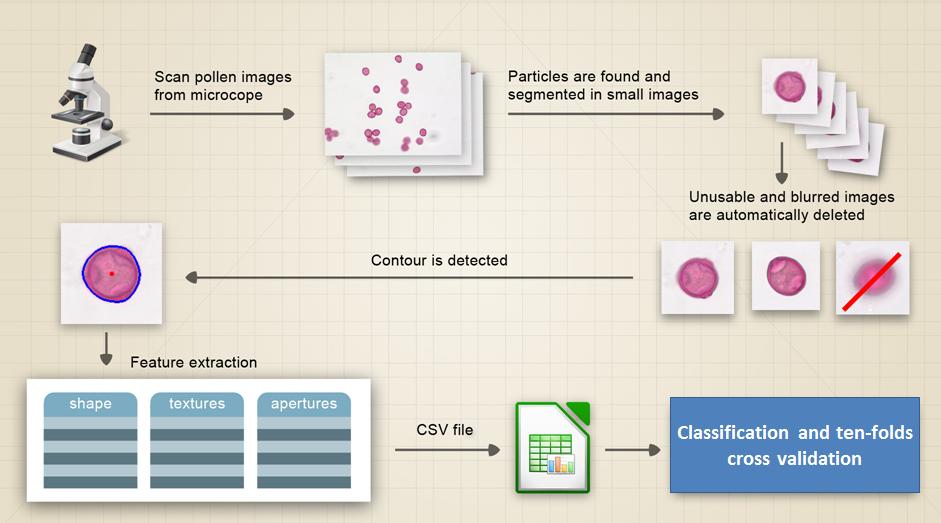
\includegraphics[width=1\columnwidth]{figures/Process1/Process1.png}
\caption{\label{fig:process}
Pollen image acquisition and classification process%
}
\end{center}
\end{figure}

\section{Image Acquisition and Particle Segmentation}

Five different species (Alder, Birch, Hazel, Mugwort, and Sweet Grass) have been stained and prepared on glass slides for use with a common digital bright-field microscope. In order to build a robust model, all species had sample images derived from three distinct laboratory slides (using a total of 600 sample images obtained from 15 different slides).
  
  
  
  
  
  
  

\begin{figure}[h!]
\begin{center}
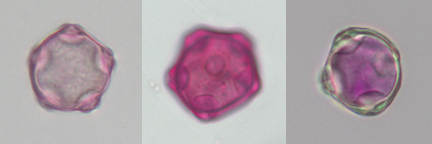
\includegraphics[width=0.7\columnwidth]{figures/3example/3example.png}
\caption{\label{fig:trainingImages}
Diverse image types, all example data used for training the Alder class of pollen}
\end{center}
\end{figure}

For particle segmentation, each digital image is processed in order to locate and segment out a confining square surrounding a pollen particle. First, a median blur and Gauassian blur are applied to a negative of the image in order to remove smaller particles that are background noise (often dirt or imperfections on the background). 
Next, a threshold is applied to the image, using the OTSU algorithm to automatically detect the histogram peak. The returned image is an optimized binary image. A second set of filters is then applied using morphological operators (iterations of erosions and dilations) to fill in the particle area. Finally, the image is converted to have a white background in preparation for further processing steps.
  
  
  
  
  
  


A blob detection algorithm is now applied in order to extract a small image surrounding each particle. This algorithm is based on four attributes {\textendash} Area, Circularity, Convexity and Inertia Ratio, with parameters for {\textquotedblleft}minimum{\textquotedblright} and {\textquotedblleft}maximum{\textquotedblright} values for each. By setting the parameters for the expected characteristics of pollen grains, the smaller images are then found and extracted.


The last filter used on the resulting images of particles is depicted in Figure \ref{fig:clearness}. Because the pollen grains settle into the slide adhesive at different depths, some particles will be out of focus. These blurry images will provide insufficient data especially concerning texture features, therefore we remove them from our analysis. A blur detection algorithm was developed and applied to each image: a Laplacian filter set to a manually determined threshold value determines which images are too blurry and removed from further processing steps. 

Lastly, the contour surrounding each pollen particle is identified, using OpenCV's \verb|findContours()| method. 

  
  
  
  

\begin{figure}[h!]
\begin{center}
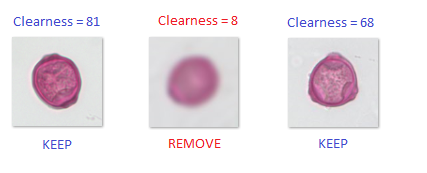
\includegraphics[width=0.7\columnwidth]{figures/clear example/clear example.png}
\caption{\label{fig:clearness}
Blur detection example
  %
}
\end{center}
\end{figure}

\section{Feature Extraction}

\subsection{Shape features}

We have used 18 shape features already identified to be useful through previous iterations of our research \cite{Lozano_2014}. The 18 selected were based on the research of developing an identification process for the Urticaceae family of pollen \cite{RodriguezDamian_2006}, as well as research into developing universal shape descriptors \cite{Costa_2009}.

Shape features used:

\begin{description}
\item[Perimeter ($P$)] Length of contour given by OpenCV's \verb|arcLength()| function
\item[Area ($A$)] Number of pixels contained inside the contour
\item[Roundness ($R$)] $4\pi A \over P^2$
\item[Compactness] $1 \over R$
\item[Roundness/Circularity Ratio ($RC$)] Another measure of roundness, see \cite{OHiggins} $P-\sqrt{P^2-4\pi A} \over P+\sqrt{P^2-4\pi A}$
\item[Mean Distance ($\bar{S}$)] Average of the distance between the center of gravity and the contour
\item[Minimum Distance ($S_{min}$)] Smallest distance between the center of gravity and the contour
\item[Maximum Distance ($S_{max}$)] Longest distance between the center of gravity and the contour
\item[Ratio1 ($R_1$)] Ratio of maximum distance to minimal distance $S_{max} / S_{min}$
\item[Ratio2 ($R_2$)] Ratio of maximum distance to mean distance $S_{max} / \bar{S}$
\item[Ratio3 ($R_3$)] Ratio of minimum distance to mean distance $S_{min}/ \bar{S}$
\item[Diameter ($D$)] Longest distance between any two points along the contour
\item[Radius Dispersion ($RD$)] Standard deviation of the distances between the center of gravity and the contour
\item[Holes ($H$)] Sum of differences between the Maximum Distance and the distance between center of gravity and the contour
\item[Euclidean Norm ($EN_2$)] Second Euclidean Norm
\item[RMS Mean] RMS mean size
\item[Mean Distance to Boundary] Average distance between every point within the area and the contour
\item[Complexity ($F$)] Shape complexity measure based on the ratio of the area and the mean distance to boundary
\end{description}



  
  
  
  
  
  
  
  
  
  
  
  
  
  
  
  
  
  

\subsection{Texture feature extraction}

A variety of texture features were selected due to their performance in prior research \cite{RodriguezDamian_2006,Redondo_2015,Maillard_2003,Marcos_2015}.
The texture features extracted included: Gabor Filters (GF), the Fast Fourier Transform (FFT), the Local Binary Pattern (LBP), the Histogram of Oriented Gradients (HOG), and Haralick features.

\subsubsection{Gabor Filters}

Gabor filters have been proven useful in image segmentation and texture analysis \cite{Zheng_2004}. The Gabor Filter function consists of the application of 5 different size masks and 8 orientation masks (See Figure \ref{fig:gabor}) in order to produce output images. For each of the 40 resulting images, we calculate the local energy over the entire image (the sum of the square of the gray-level pixel intensity), and the mean amplitude (the sum of the amplitudes divided by the total number of images). In addition to these 80 values, we also store the total local energy for each of the 8 directions as well as the direction where the local energy is at the maximum.

  
  
  
  
  
  
  
  
  
  
  
  

\begin{figure}[h!]
\begin{center}
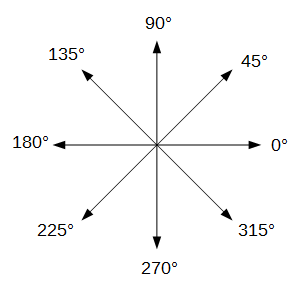
\includegraphics[width=0.42\columnwidth]{figures/direction1/direction1.PNG}
\caption{\label{fig:gabor}
The 8 directions of the mask for the Gabor Filters
  %
}
\end{center}
\end{figure}


\subsubsection{Fourier Transform}

Fourier Transforms translate an image from the spatial domain into the frequency domain, and are useful because lower frequencies represent an area of an image with consistent intensity (relatively featureless areas) and higher frequencies represent areas of change \cite{Haas_2011}. Just as in spatial analysis, we cannot compare images directly, but first need to extract features. In the frequency domain, we likewise extract useful information through analysis of frequency peaks. Here, we apply a Fast Fourier Transform to the image, apply a logarithmic transformation, and create a graph of the resulting frequency domain. After taking the highest 10 frequency peaks, we compute the differences between the peaks and store these values, as well as the mean of the differences and the variance of the differences. 

    
  
  
  
  


\subsubsection{Haralick Features}

Haralick features \cite{Haralick_1973} are determined by computations over the GLCM (Grey-Level Co-Occurence Matrix). Here, we use: the \emph{angular second moment}, \emph{contrast}, \emph{correlation}, \emph{sum of squares: variance}, \emph{inverse difference moment}, \emph{sum average}, \emph{sum variance}, \emph{sum entropy}, \emph{entropy}, \emph{difference variance}, \emph{difference entropy}, \emph{measure of correlation 1}, and \emph{measure of correlation 2}. These are 13 out of the 14 original features developed by Haralick: the 14th is typically left out of computations due to uncertainty in the metric's stability. 

\subsubsection{Histogram oriented gradient (HOG)}

The Histogram of Oriented Gradients is calculated by first determining gradient values over a 3 by 3 Sobel mask. Next, bins are created for the creation of cell histograms; here, 10 bins were used. The gradient angles are divided into these bins, and the gradient magnitudes of the pixel values are used to determine orientation. After normalization, the values are flattened into one feature vector. 

\subsubsection{Local Binary Pattern (LBP)}

To obtain local binary patterns, a 3 by 3 pixel window is moved over the image, and the value of the central pixel is compared to the value of its neighbors. In the case that the neighbor is of lower value, it is assigned a zero, and in the case of a higher value, a one. This string of eight numbers ("00011101" for instance) is the determined local pattern. The frequency of the occurrence of each pattern is used as the texture description. 
  
  

  
  
  
  
  
  
  

\begin{figure}[h!]
\begin{center}
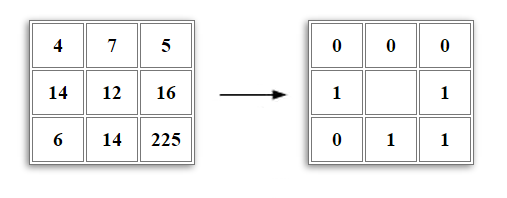
\includegraphics[width=0.42\columnwidth]{figures/is/is.png}
\caption{\label{fig:lbp_grid}
Example output for Local Binary Patterns%
}
\end{center}
\end{figure}

\begin{figure}[h!]
\begin{center}
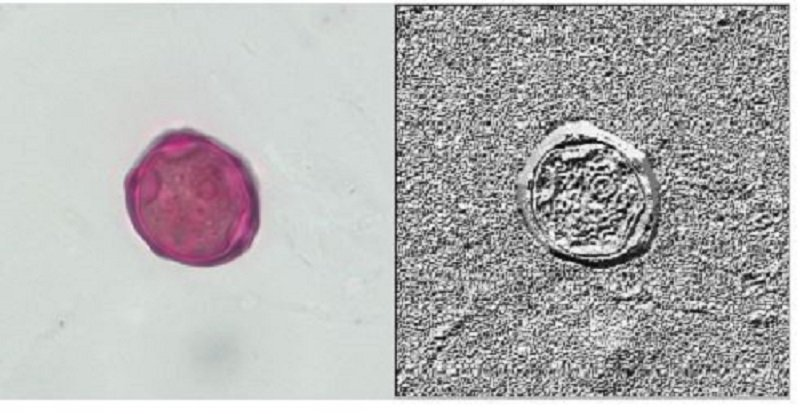
\includegraphics[width=0.7\columnwidth]{figures/comparer_lbp1/comparer_lbp1.jpg}
\caption{\label{fig:lbp_output}
Local Binary Pattern function applied to pollen image%
}
\end{center}
\end{figure}

\subsubsection{Aperture Detection}

The number and type of apertures present on the pollen surface is a typical feature used by palynologists in order to determine the pollen species. Therefore, it seems useful to also build an automatic aperture detection function in order to identify and count apertures as an addition feature set. Preliminary work identifying apertures \cite{Lozano_2013_ICIAP} has shown potential for this analysis.
First, a moving window segments the pollen image into smaller areas. Each smaller image is manually labeled as an aperture or not an aperture. Texture features are extracted from these smaller images, including those through a Fast Fourier Transform (FFT), Gabor Filters (GF), Local Binary Pattern (LBP), Histogram of Oriented Gradients (HOG), and Haralick features. A supervised learning process (through the use of support vector machines) then creates a model for each of the four species expected to include apertures on the surface.
Once an unlabeled pollen image is given to be classified, the system again uses a moving window to break up the image into subsections. These smaller sections are then loaded into the generated model, and four values are returned for each detected aperture, corresponding to the probability that the aperture is of type Alder, Birch, Hazel, and Mugwort. 

    
    
  
  
  
  
  
  
  

\begin{figure}[h!]
\begin{center}
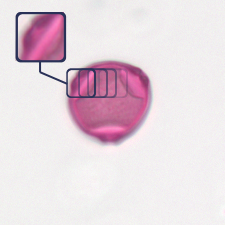
\includegraphics[width=0.7\columnwidth]{figures/birchMod/birchMod.png}
\caption{\label{fig:aperture_window}
Window moving all over the pollen%
}
\end{center}
\end{figure}

\begin{figure}[h!]
\begin{center}
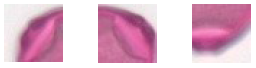
\includegraphics[width=0.7\columnwidth]{figures/apertures/apertures.PNG}
\caption{\label{fig:aperture_detection}
Apertures detected by the program on a Birch pollen%
}
\end{center}
\end{figure}

\section{Classification}

Once the shape, texture, and aperture features have been calculated, they are added together into a csv file. A data set of 5 species with 40 sample pollen images from 3 separate sample slides led to a total of 600 samples, each with 252 extracted features. A supervised learning process used this data for model creation, which was then tested using ten-fold cross validation. Both support vector machines and a random forest classifier showed promising (and very similar results); for the results reported here a random forest classifier was used due to faster processing on the larger data sets. The n-estimators parameter for this method was set to a typical size of 100 (increasing this number did lead to slightly improved results yet also dramatically increased processing times).
    
  
  
  
  

\section{Results}

Using a random forest classifier on a total of 600 samples (120 each for each species) and 252 features, a model was generated with an accuracy of $87\% \pm 2\%$. Considering that the samples were intentionally selected for variability in their appearance and background (See Figure \ref{fig:trainingImages}), this is an indication of a robust, reliable model that shows promise for expansion in the future to also include datasets collected from an outdoor environment. 

The dataset was further modified into different versions in order to test the results using only subsets of the features available.

\begin{table}
    \centering
        \begin{tabular}{ l c }
            \toprule
            Features & Accuracy \\ \midrule
            Shape features & $64\% \pm 3\%$ \\ 
            Shape and Gabor & $76\% \pm 2\%$ \\ 
            Shape and FFT & $65\% \pm 2\%$ \\ 
            Shape and LBP & $65\% \pm 3\%$ \\ 
            Shape and HOG & $67\% \pm 2\%$ \\ 
            Shape and Haralick & $87\% \pm 3\%$ \\ 
            Shape and Aperture & $67\% \pm 2\%$ \\
            \bottomrule
        \end{tabular}
\end{table}

The above table shows the accuracies of the trained models. Using only the 18 shape features, an accuracy of $64\% \pm 3\%$ was achieved, and adding texture information either through Gabor Filters or Haralick features substantially improved the results.

  
  
  
  
  
  
  
  
  
  
  
  
  
  
  
  
  
  
  
  
  
  

\section{Conclusion}

Through this research, we have tested an expanded sample set of 5 species of pollen particles and used shape, texture and aperture features for use in classification. Use of all features led to an accuracy of $87\% \pm 2\%$. Through testing of individual texture features in combination with shape features, it was found that using only the shape and Haralick features resulted in an accuracy of $87\% \pm 3\%$. Gabor Filters also proved to be a useful feature as seen through the improved accuracy compared to using just the shape features alone. Surprisingly, the other texture features as well as the aperture features did not result in significant accuracy gains. One next step of research would be to investigate under which exact conditions certain texture features prove useful. In the case of the aperture features, one known limitation is that the aperture types were trained on a more limited dataset. Because the aperture detection process technique developed did have positive results in determining correct aperture positions, it would be interesting to retrain the aperture type on a wider dataset and see if this results in a more useful set of extracted features. Future research would also include application of this process to data collected outside of a laboratory environment, as well as expansion to include more pollen species.
    
  
  
  
  
  

\bibliography{bibliography/biblio.bib}

\end{document}

